\documentclass[a4paper,12pt]{article}\usepackage[]{graphicx}\usepackage[]{color}
%% maxwidth is the original width if it is less than linewidth
%% otherwise use linewidth (to make sure the graphics do not exceed the margin)
\makeatletter
\def\maxwidth{ %
  \ifdim\Gin@nat@width>\linewidth
    \linewidth
  \else
    \Gin@nat@width
  \fi
}
\makeatother

\definecolor{fgcolor}{rgb}{0.345, 0.345, 0.345}
\newcommand{\hlnum}[1]{\textcolor[rgb]{0.686,0.059,0.569}{#1}}%
\newcommand{\hlstr}[1]{\textcolor[rgb]{0.192,0.494,0.8}{#1}}%
\newcommand{\hlcom}[1]{\textcolor[rgb]{0.678,0.584,0.686}{\textit{#1}}}%
\newcommand{\hlopt}[1]{\textcolor[rgb]{0,0,0}{#1}}%
\newcommand{\hlstd}[1]{\textcolor[rgb]{0.345,0.345,0.345}{#1}}%
\newcommand{\hlkwa}[1]{\textcolor[rgb]{0.161,0.373,0.58}{\textbf{#1}}}%
\newcommand{\hlkwb}[1]{\textcolor[rgb]{0.69,0.353,0.396}{#1}}%
\newcommand{\hlkwc}[1]{\textcolor[rgb]{0.333,0.667,0.333}{#1}}%
\newcommand{\hlkwd}[1]{\textcolor[rgb]{0.737,0.353,0.396}{\textbf{#1}}}%
\let\hlipl\hlkwb

\usepackage{framed}
\makeatletter
\newenvironment{kframe}{%
 \def\at@end@of@kframe{}%
 \ifinner\ifhmode%
  \def\at@end@of@kframe{\end{minipage}}%
  \begin{minipage}{\columnwidth}%
 \fi\fi%
 \def\FrameCommand##1{\hskip\@totalleftmargin \hskip-\fboxsep
 \colorbox{shadecolor}{##1}\hskip-\fboxsep
     % There is no \\@totalrightmargin, so:
     \hskip-\linewidth \hskip-\@totalleftmargin \hskip\columnwidth}%
 \MakeFramed {\advance\hsize-\width
   \@totalleftmargin\z@ \linewidth\hsize
   \@setminipage}}%
 {\par\unskip\endMakeFramed%
 \at@end@of@kframe}
\makeatother

\definecolor{shadecolor}{rgb}{.97, .97, .97}
\definecolor{messagecolor}{rgb}{0, 0, 0}
\definecolor{warningcolor}{rgb}{1, 0, 1}
\definecolor{errorcolor}{rgb}{1, 0, 0}
\newenvironment{knitrout}{}{} % an empty environment to be redefined in TeX

\usepackage{alltt}
\usepackage[margin=1in]{geometry}
\usepackage[utf8]{inputenc}
\usepackage{times}
\usepackage{booktabs}
\usepackage{natbib}
\usepackage{amsmath}
\usepackage{setspace}
\renewcommand{\thefigure}{S\arabic{figure}}
\usepackage[normalem]{ulem}
\usepackage{sectsty}
\subsectionfont{\normalfont\large\underline}

\title{Measuring Subgroup Preferences in Conjoint Experiments}
\author{Sara Hobolt, Thomas J. Leeper, and James Tilley}
\IfFileExists{upquote.sty}{\usepackage{upquote}}{}
\begin{document}

\maketitle

{\abstract Conjoint analysis has experienced a recent resurgence. The driving force for this change has been the introduction by \citet{HainmuellerHopkinsYamamoto2014} of a fully randomized conjoint design and an associated analytic approach that emphasizes a single causal quantity of interest: namely, the average marginal component effect (AMCE). The AMCE convey the degree to which a given value of a feature increases or decreases respondents' support for a conjoint profile, averaging across all respondents and all other profile features. While randomization of profile features gives the AMCE a causal interpretation, most published conjoint analyses use AMCEs for descriptive purposes: that is, not map variation in preferences across attributes of a multidimensional object, such as a candidate individual or public policy. And many authors also engage in subgroup analyses, wherein they compare subsets of respondents to one another with respect to AMCEs. This paper argues that such approaches can substantially mislead researchers about the degree of agreement or disagreement between subgroups, demonstrates the problem using several example datasets, and provides several suggestions for improved reporting and interpretation. Most importantly, it highlights that the difference in AMCEs between groups is sensitive to the choice of reference categories of features, while the difference in the marginal means is not sensitive in this way. When groups substantially differ in preferences, the difference in marginal means rather than the difference better conveys the size of such disagreements.}










\clearpage


Conjoint analysis has experienced a recent resurgence in the social sciences and especially in political science. The driving force has been the introduction by \citet{HainmuellerHopkinsYamamoto2014} of a fully randomized conjoint design and an associated analytic approach that emphasizes a single quantity of interest: namely, the average marginal component effect (AMCE). By capturing the multidimensionality of target objects, such as a candidate individual or public policy, the conjoint design breaks any explicit or implicit confounding between those features, thus giving the AMCE a clear causal interpretation: the degree to which a given value of a feature increases or decreases respondents' support for a packaged conjoint profile, averaging across all respondents and all other profile features.

While randomization of profile features gives the AMCE a causal interpretation, most published conjoint analyses use AMCEs for descriptive purposes: that is, to map variation in preferences across attributes of a multidimensional object. This is particularly the case when researchers engage in subgroup analyses of conjoint experiments. For example, \citet{HainmuellerHopkinsYamamoto2014} perform a subgroup analysis on their immigration experiment in which they perform a median split on a measure of ethnocentrism and then compare AMCEs for the two subgroups.\footnote{This is achieved by subsetting the data based upon the measure of ethnocentrism and performing separate regressions for high- and low-ethnocentrism respondents.} The interpretation therefore focuses not just on the arbitrarily signed AMCEs within each subgroup (what Hainmueller et al. term ``conditional AMCEs''; 13) but also on an implied quantity of interest: the difference between conditional AMCEs. The difference in AMCEs is then used to \textit{descriptively} interpret apparent differences in preferences between the two groups. Yet what is not obvious in such analyses is that differences-in-preferences are not directly reflected in such differences-in-AMCEs. Indeed, where preferences between the groups are similar, the difference in AMCEs can be large and where preferences diverge, the difference-in-AMCEs can be small. This is because the AMCE as a quantity of interest calculated against an arbitrarily chosen reference category for each factor level; where preferences between subgroups diverge in the reference category, the difference-in-AMCEs mislead about underlying preferences.

In what follows, we formalize this problem of reference category choice and demonstrates how it is especially problematic when researchers engage in the now-common practice of comparing conditional AMCEs across respondent subgroups. The paper then demonstrates the problem using several example datasets and provides suggestions for improved reporting and interpretation based around a purely descriptive quantity of interest: namely, the unadjusted marginal means. Software for the R programming language that can be used to examine sensitivity of conjoint analysis to reference category selection and to calculate marginal means (as well as AMCEs) is also discussed.


\section{Quantities of Interest}\label{sec:quantities}

% AMCE
\begin{knitrout}
\definecolor{shadecolor}{rgb}{0.969, 0.969, 0.969}\color{fgcolor}\begin{kframe}


{\ttfamily\noindent\itshape\color{messagecolor}{\#\# Loading required namespace: ggstance}}\end{kframe}\begin{figure}
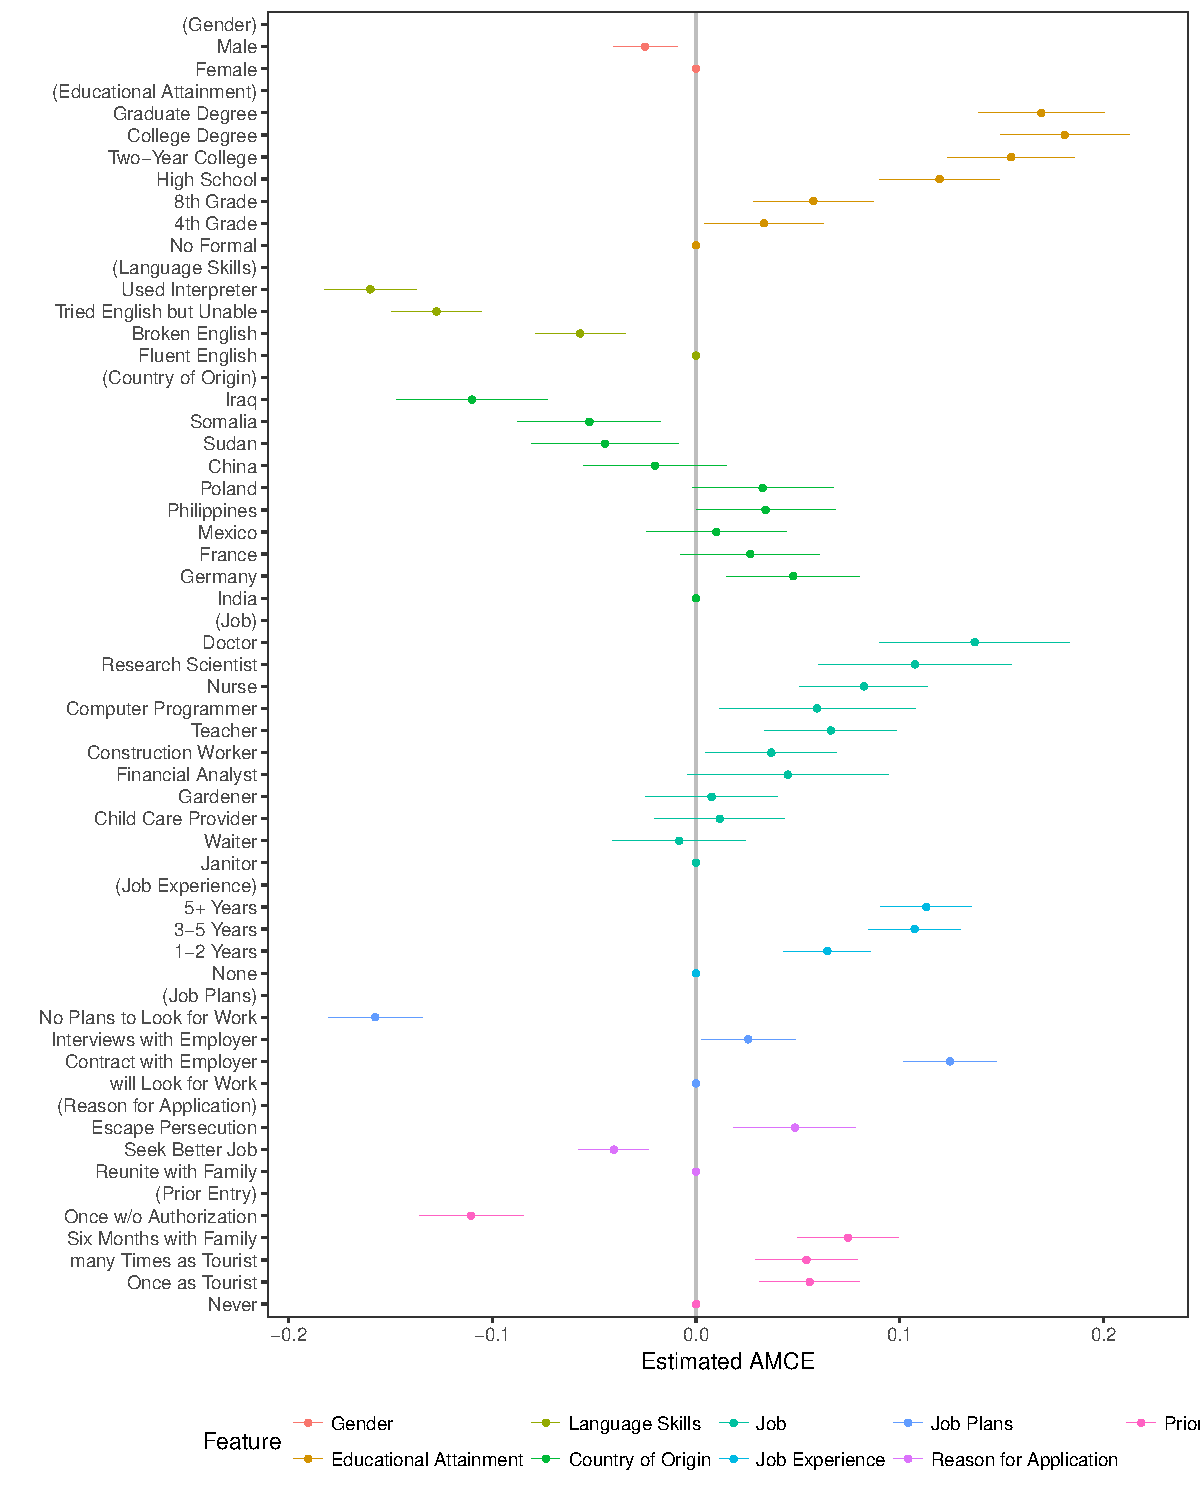
\includegraphics[width=\maxwidth]{figure/hainmueller_immigration-1} \caption[Replication of Hainmueller et al]{Replication of Hainmueller et al. (2014) Results}\label{fig:hainmueller_immigration}
\end{figure}


\end{knitrout}

A fully randomized conjoint design (without constraints between profile features) is simply a full-factorial experiment. The ways of analyzing this experiment are numerous, including various forms of linear model statistics such pairwise comparisons between cell or factor means, linear regression, ANOVA, and so forth. In this section, we describe four quantities of interest that arise when analysing conjoint designs: average marginal component effects (AMCEs), conditional AMCEs, differences in conditional AMCEs, and marginal means. We discuss each in turn.

First, in the \citet{HainmuellerHopkinsYamamoto2014} approach, the quantity of interest is shifted from the traditional linear model statistics used in traditional analysis of factorial experiments to a statistic nearly equivalent to the average marginal effect of each profile feature level, namely the \textit{average marginal component effect} (AMCE). In a fully randomized design, this statistic is equivalent to the average marginal effect of each feature level for a model where each feature is converted into a matrix of indicator variables for each level with one left out as a reference category.\footnote{In designs that entail constraints between profile features, the average marginal effect is a weighted average of effects across each combination of the constrained features where the weights of the effects are the design (display) probabilities of the feature combinations.}

As an example, Figure \ref{fig:hainmueller_immigration} provides a replication of Hainmueller et al.'s (2014) results, showing the AMCEs for each experiment. The AMCEs provide for both causal and descriptive inferences. Because features are randomly assigned to respondents, differences in evaluations of profiles that vary according to a given feature are causally interpretable as the effect of that randomly assigned profile variation. Yet while randomization of profile features gives the AMCE a causal interpretation, most published conjoint analyses use AMCEs for descriptive purposes: that is, to map variation in preferences across attributes of a multidimensional object. For example, \citet{HainmuellerHopkinsYamamoto2014} describe some of the results of their conjoint analysis of congressional candidate preferences:

\begin{quote}
We also see a bias against Mormon candidates, whose estimated level of support is 0.06 (SE = 0.03) lower when compared to a baseline candidate with no stated religion. Support for Evangelical Protestants is also 0.04 percentage points lower (SE = 0.02) than the baseline. Mainline Protestants, Catholics, and Jews all receive ratings indistinguishable from those of a baseline candidate. (19)
\end{quote}

This characterization of the results has a distinctly descriptive flavor. While a given religious characteristic \textit{causes} respondents to evaluate a given candidate more or less favorably, the gist of the analysis is that there are differences in the evaluations of candidates of different religious persuasions. \citeauthor{HainmuellerHopkinsYamamoto2014}'s phrasing highlights another feature of conjoint analysis that is not widely discussed: the baseline (or reference category) in the estimation of AMCEs significantly colors which pairwise comparisons between features are highlighted and the degree to which preferences are stated in positive or negative terms. By choosing a non-religious candidate as a baseline, the AMCEs are all expressed relative to this baseline; the difference (if any) between evaluations of Mormon and Evangelical candidates, for example, is not obvious and while it is likely that Mainline Protestant, Catholic, and Jewish candidates are all preferred over Mormon or Evangelical candidates, the AMCEs for these categories are indistinguishable from zero (rather than the positive values they would take if Mormon or Evangelical were the reference category). Similarly, by selecting a reference category that receives middling support (i.e., more favorability than some other feature levels but less favorability than others), some AMCEs are positive while others are negative. Yet because any feature level could be used as the reference cateory, the size but also \textit{direction} of AMCEs is arbitrary. Were the category with the lowest favorability chosen as the reference, all AMCEs would be positive; were the category with the highest favorability chosen as the reference, all AMCEs would be negative. The results would be \textit{numerically equivalent} --- because ultimately the choice of reference category is completely arbitrary and mathematicaly irrelevant --- but the choice as sizable consequences for the interpretation of conjoint analyses. We return to this issue below.


% Difference in conditional AMCEs
\begin{table}
\caption{Uses of Subgroup Analysis in Published Work}\label{tab:papers}
\begin{center}
\footnotesize
\begin{tabular}{p{2.5in} p{2in} p{2in}}\toprule
\textbf{Paper} & \textbf{Topic} & \textbf{Subgroup Comparisons} \\ \midrule
Hainmueller, Hopkins, and Yamamoto (2014) & Immigration Preferences & Ethnocentrism \\
Bechtel and Scheve (2013) & Climate agreement preferences & Environmentalism and International Reciprocity Attitudes \\
Bechtel, Genovese, and Scheve (2017) & Climate agreement preferences & Employment sector emissions \\
Hansen, Olsen, and Bech (2015) & Policy Preferences & Partisanship \\
Carlson (2015) & Candidate Choice & Co-ethnicity \\
Franchino and Zucchini (2015) & Candidate Choice & Political Interest, Left-right self-placement\\
Carnes and Lupu (2016) & Candidate Choice & Partisanship \\
Mummolo (2016) & News Selection & Various\\
Mummolo and Nall (2016) & Mobility preferences & Partisanship \\
Ballard-Rosa, Martin, and Scheve (2016) & Tax Preferences & Various\\
Bechtel, Hainmueller, and Margalit (2017) & International bailout preferences & Various\\
Sen (2017) & Judicial candidate preferences & Partisanship \\
Campbell, Cowley, Vivyan, and Wagner (2016) & Candiate preferences & Partisanship \\
Kirkland, Coppock (2017) & Candidate choice & Partisanship \\ \bottomrule
\end{tabular}
\end{center}
\end{table}

Second, in practice, researchers do not only analyze conjoint designs using the AMCE statistic for the sample as a whole. They also frequently report \textit{conditional} AMCEs, wherein AMCEs are calculated separately for subgroups of respondents and those conditional estimates are directly compared. Table \ref{tab:papers} reports a list of recent published articles in political science that engage in this form of subgroup analysis.\footnote{\citet{RatkovicTingley2017} considered efficient methods for performing subgroup analyses in conjoint designs. Our focus here is on the narrower problem of interpreting subgroup analyses as traditionally performed.}

Third, while analyzing subgroup preferences is in principle unproblematic, the comparison of subgroup conditional AMCEs involves an implied quantity of interest that \citet{HainmuellerHopkinsYamamoto2014} did not explicitly discuss: namely, the \textit{difference-in-AMCEs}. For example, in one analysis \citet{HainmuellerHopkinsYamamoto2014} eyeball the pattern of AMCEs among high- and low-ethnocentrism respondents and interpret that ``the patterns of support are generally similar for respondents irrespective of their level of ethnocentrism'' (22). The difference in AMCEs is thus used as a way of characterizing differences in underlying preferences between groups. While AMCEs do provide insight into the descriptive variation in preferences within-group and across-features, this act of interpretation is not necessarily valid between-groups. This is an issue we return to below.


% Marginal means
Finally, an alternative quantity of interest in any experiment (but one not discussed by \citealt{HainmuellerHopkinsYamamoto2014}) is the treatment group mean outcome. Comparisons of this quantity of interest across experimental conditions ultimately underlies causal inference yet it is not widely used in conjoint analysis. One reason for this is that the high-dimensionality of conjoint designs --- and the resulting data sparsity --- means that it is not typically possible to calculate mean outcomes for every possible combination of feature levels.

Yet traditional analysis of factorial experiments provides a closely related measure that leverages the independent randomization of experimental factors to provide a useful insight into the distribution of outcomes across levels of each feature. This \textit{marginal mean} is, in essence, the mean outcome in each treatment condition taking factors one-at-a-time; in the case of conjoint designs, this means examining the mean outcome when a given feature level is present versus not present. In conjoint designs, the marginal mean outcome for a given feature level is a descriptively useful quantity that conveys the preferences of respondents toward profiles that have that feature level, averaging across co-occurrences with levels of all other features. In a forced-choice design, this quantity can be read as: given a profile contains level $x_i$ of feature $x$, the proportion of times respondents choose that profile is the marginal mean for that feature level. In forced choice designs (with two alternatives), this bounds the marginal means between 0 and 1 with the further constraint that the average of marginal means for levels of a given factor is definitionally equal to 0.5.\footnote{It is not possible for the marginal mean to ever equal zero or one if it possible for pairs of profiles shown together to both have the same level of a given feature (for example, both immigrants are from Germany). Instead, the marginal mean can range from the probability of co-occurrence to 1 minus that probability. If there are five levels of a feature, each shown with equal probability, then $Pr(Co-occurrence) = \frac{1}{5}*\frac{1}{5} = 0.04$ such that the marginal mean can take values in the range $(0.04,0.96)$. If the design is constrained so that features cannot be the same for both immigrants, then the marginal means fully range from zero to one.} In non-forced designs, the marginal means can vary arbitrarily along the outcome scale used.

\begin{knitrout}
\definecolor{shadecolor}{rgb}{0.969, 0.969, 0.969}\color{fgcolor}\begin{kframe}


{\ttfamily\noindent\itshape\color{messagecolor}{\#\# Loading required namespace: ggstance}}\end{kframe}\begin{figure}
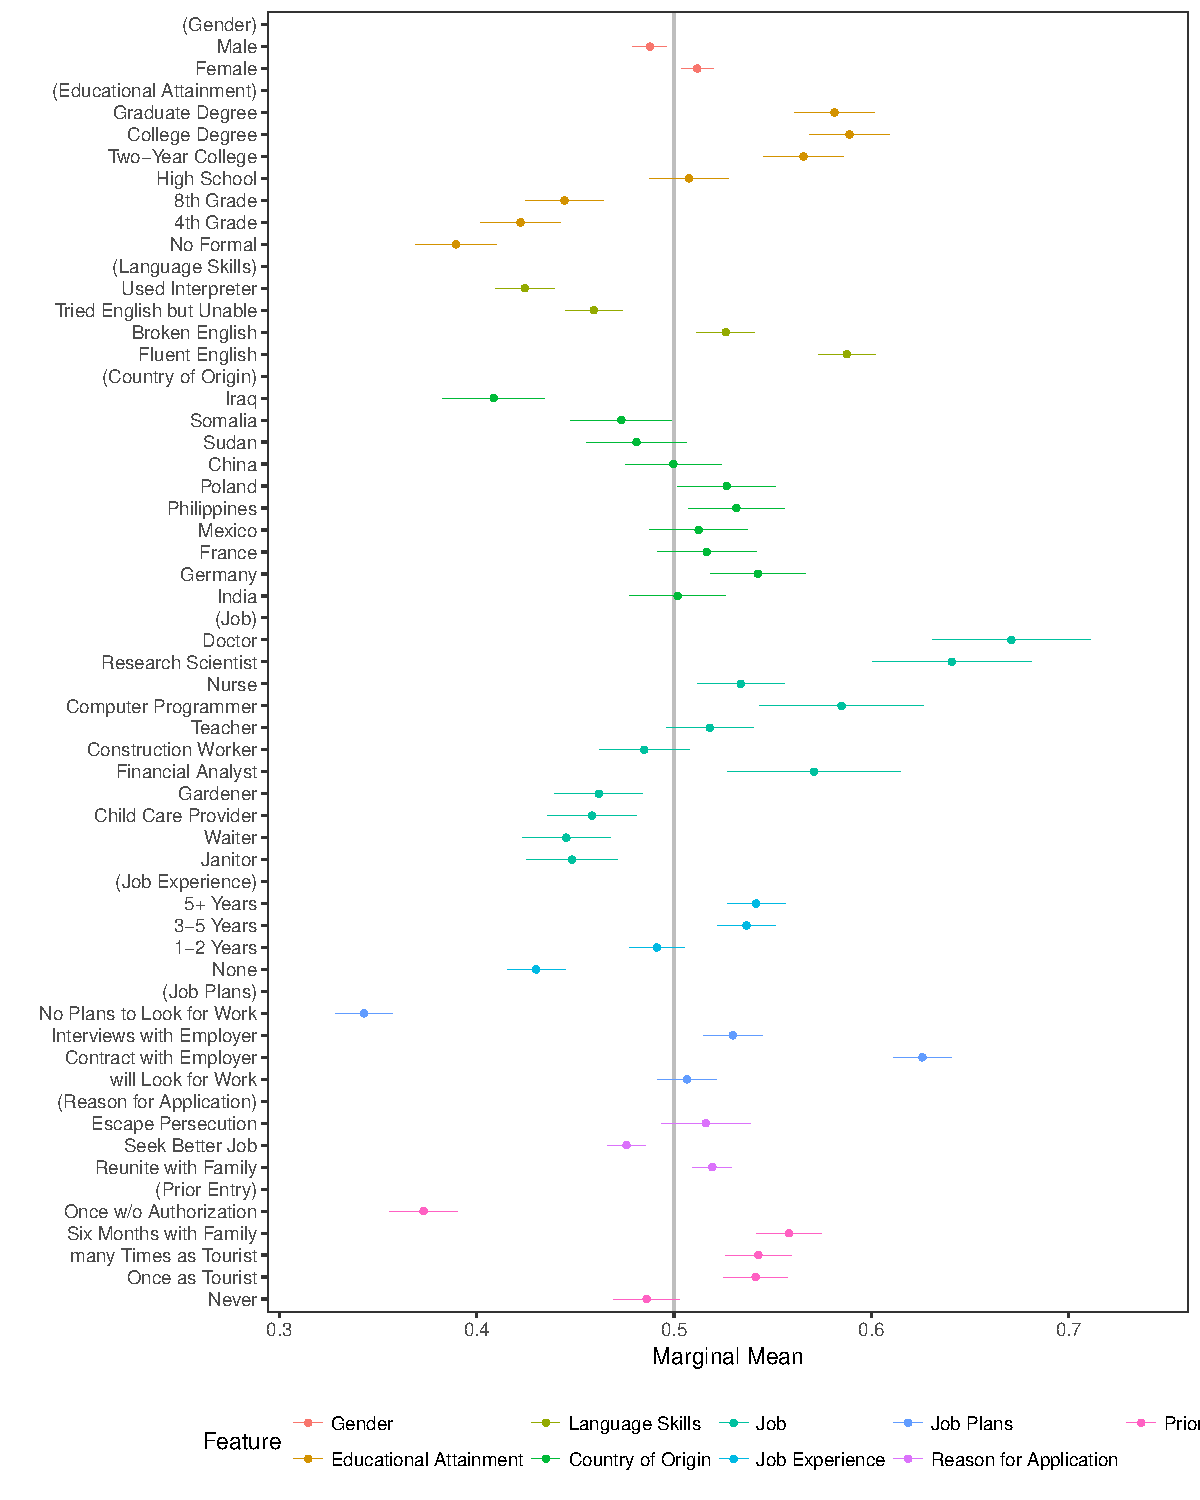
\includegraphics[width=\maxwidth]{figure/hainmueller_immigration_mm-1} \caption[Replication of Hainmueller et al]{Replication of Hainmueller et al. (2014) using Marginal Means}\label{fig:hainmueller_immigration_mm}
\end{figure}


\end{knitrout}

As an example, Figure \ref{fig:hainmueller_immigration_mm} shows marginal means for the immigration experiment from \citet{HainmuellerHopkinsYamamoto2014}. The results provide a close visual analogue to the AMCEs shown in Figure \ref{fig:hainmueller_immigration}. The differences are, however, two-fold: 1) rather than a single level of feature being set aside as a reference category, marginal means (and their variances) are estimated for all levels of every feature; and 2) the marginal means vary around the grand mean of the outcome rather than around 0. In the forced-choice design used by Hainmueller et al., this means all marginal means center at 0.5.


\section{Challenges of Interpretation}\label{sec:challenges}

With quantities of interest now defined, this section describes three issues related to the focus on average marginal component effects as the main quantity of interest in the analysis of conjoint designs. First, that the selection of the reference category for each feature level is arbitrary thus leading to potential failures of intuition due to the numerical equivalence but intuitive distinctions in results using different reference categories. Second, that subgroup analyses of conjoint designs that rely upon AMCEs analytically confuse differences in conditional AMCEs with differences-in-preferences, despite their non-equivalence. And finally, that unadjusted marginal means as a quantity of interest are not susceptible to either of the preceding two concerns and therefore provide a more useful measure for describing preferences in conjoint designs than analysis based upon causally interpretable AMCEs.

\subsection{Arbitrary reference category choice}\label{sec:reference}

\begin{knitrout}
\definecolor{shadecolor}{rgb}{0.969, 0.969, 0.969}\color{fgcolor}\begin{figure}
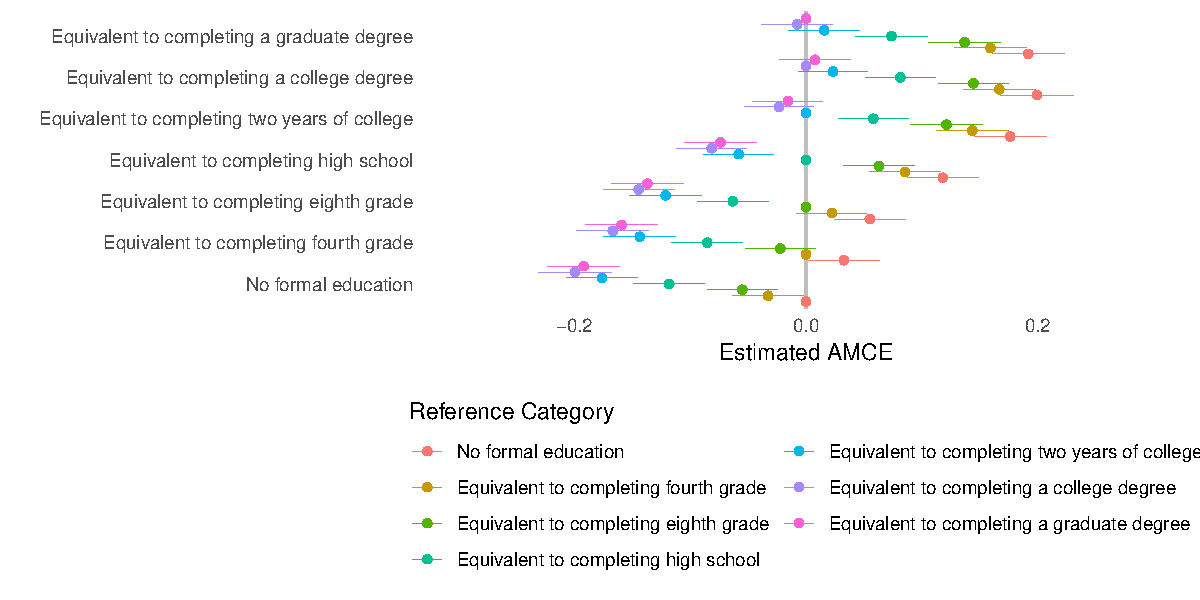
\includegraphics[width=\maxwidth]{figure/reference_category-1} \caption[Reference Category Diagnostic for the 'Country of Origin' Feature from Hainmueller et al]{Reference Category Diagnostic for the 'Country of Origin' Feature from Hainmueller et al. (2014)}\label{fig:reference_category}
\end{figure}


\end{knitrout}

\subsection{Subgroup Analysis}\label{sec:subgroup}

A conventional presentation of subgroup analyses in a conjoint design is shown in the top panel of Figure \ref{fig:subgroup_results}. Note how the conditional AMCEs for several levels --- Somalia, Sudan, China, Mexico, and Philippines --- flip signs. While both negative, it also appears that high ethnocentrism respondents are substantially more negative toward immigrants from Iraq. By contrast, the AMCEs for the two groups for immigrants from Poland, France, Germany (and India, the reference category) are quite similar. The lower panel of Figure \ref{fig:subgroup_results} shows an alternative analysis: namely, marginal means for both subgroups.

While the differences in preferences as measured by unadjusted marginal means for the two subgroups for immigrants from Somalia and Sudan do appear to differ (as reflected in the AMCEs), the differences in preferences for immigrants from Iraq, China, and the Philippines are indistinguishable from zero. Apparent similarity in the patterns of AMCE mask where and in what direction preferences for the two subgroups differ.

\begin{knitrout}
\definecolor{shadecolor}{rgb}{0.969, 0.969, 0.969}\color{fgcolor}\begin{figure}
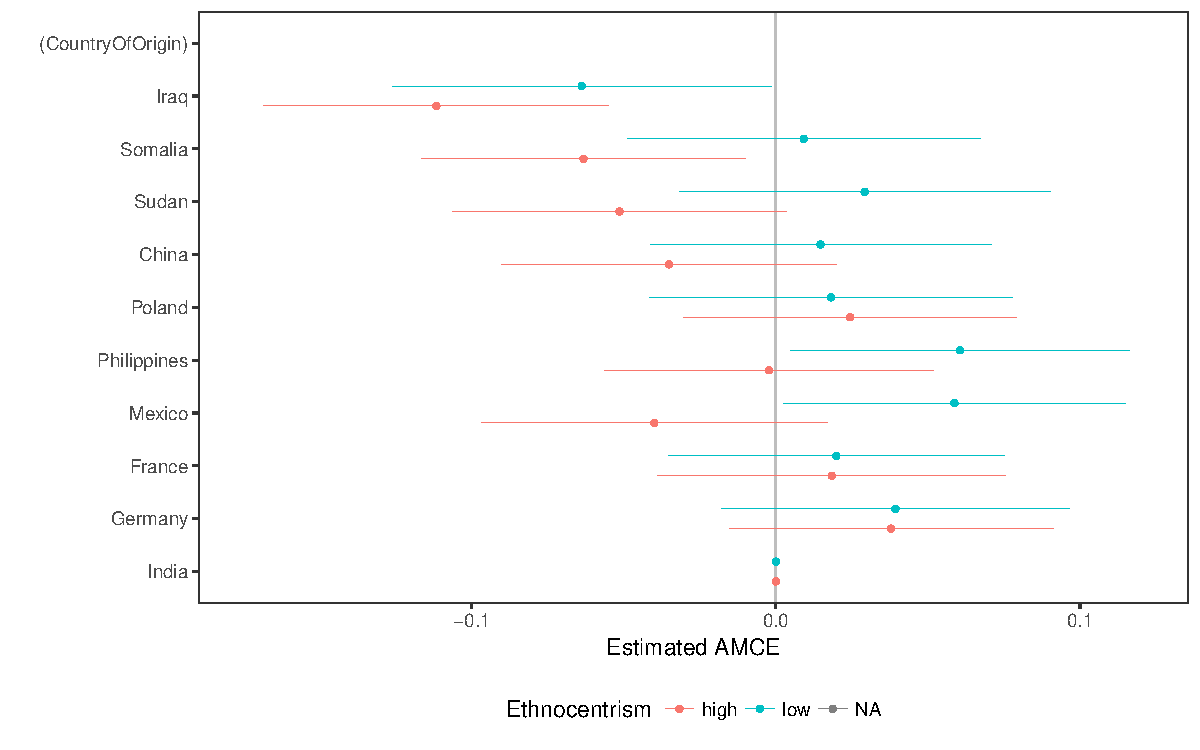
\includegraphics[width=\maxwidth]{figure/subgroup_results-1} \caption[Subgroup Analysis for the 'Country of Origin' Feature from Hainmueller et al]{Subgroup Analysis for the 'Country of Origin' Feature from Hainmueller et al. (2014)}\label{fig:subgroup_results1}
\end{figure}

\begin{figure}
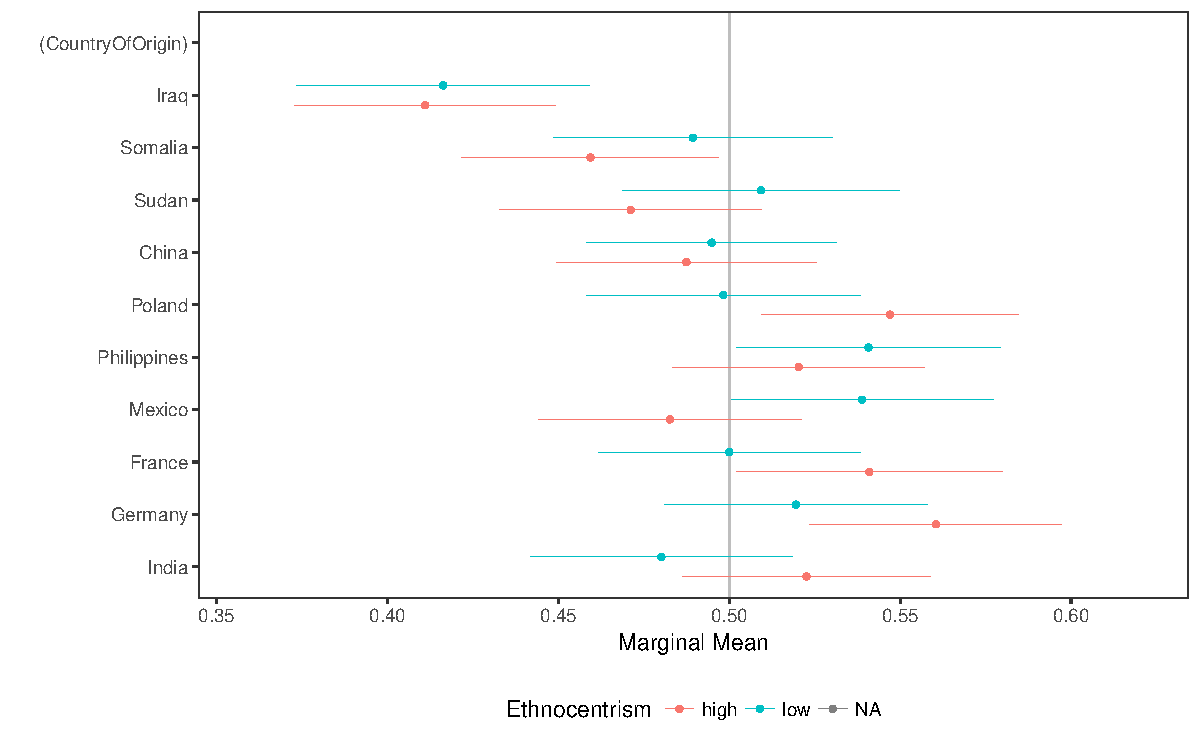
\includegraphics[width=\maxwidth]{figure/subgroup_results-2} \caption[Subgroup Analysis for the 'Country of Origin' Feature from Hainmueller et al]{Subgroup Analysis for the 'Country of Origin' Feature from Hainmueller et al. (2014)}\label{fig:subgroup_results2}
\end{figure}


\end{knitrout}

Take, for example, the fact that underlying differences in preferences between the two groups are largest for immigrants from Mexico and Poland. While low ethnocentrism respondents are indifferent about respondents from Poland, high ethnocentrism respondents favor them substantially. While low ethnocentrism are slightly favorable toward immigrants from Mexico, high ethnocentrism respondents are slightly opposed to immigrants from that country. The difference in preferences toward immigrants from Mexico is reflected in the pattern of AMCEs but the difference in preferences toward immigrants from Poland is not. Why?

\begin{knitrout}
\definecolor{shadecolor}{rgb}{0.969, 0.969, 0.969}\color{fgcolor}\begin{figure}
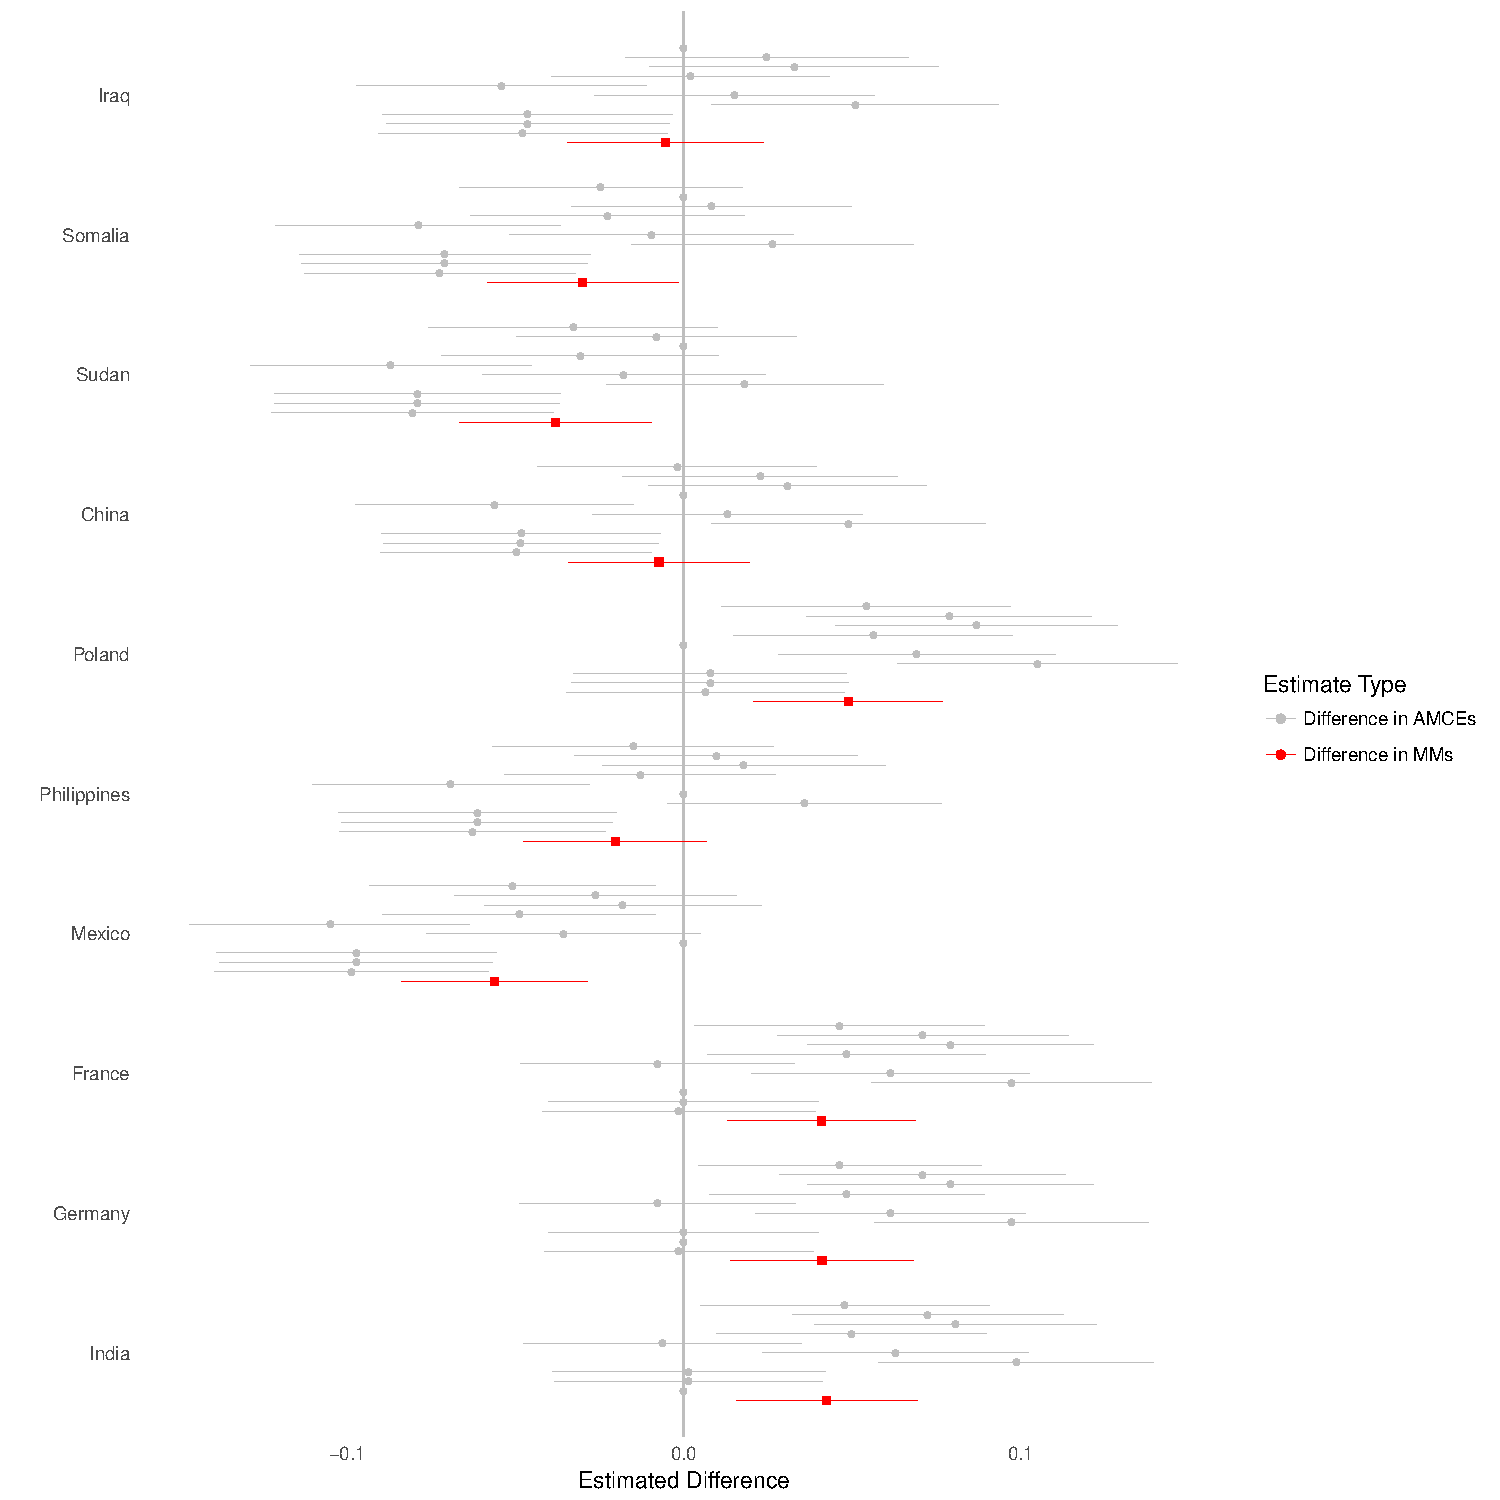
\includegraphics[width=\maxwidth]{figure/hainmueller_subgroup_differences-1} \caption[Differences in Marginal Means and AMCEs, by Ethnocentrism, from Hainmueller et al]{Differences in Marginal Means and AMCEs, by Ethnocentrism, from Hainmueller et al. (2014)}\label{fig:hainmueller_subgroup_differences}
\end{figure}


\end{knitrout}

While the difference in marginal means conveys the fixed difference in revealed preferences between the two groups, the apparent difference in preferences between groups conveyed by a difference-in-AMCEs is sensitive to the reference category chosen when estimating the effects. Figure \ref{fig:fig:hainmueller_subgroup_differences} shows the results of a diagnostic procedure for examining the sensitivity of differences-in-AMCEs to the choice of reference category. The difference in preferences as measured by marginal means for each feature level is shown in red. The differences in preferences as measured by difference-in-AMCEs are shown in gray, with the difference calculated separately for each of the 10 possible reference categories.

Thus, in the top-most set of bars (labelled ``Iraq''), the difference-in-AMCEs when Iraq is the reference category is definitionally fixed at zero and not estimated. Iterating through the other possible reference categories, the estimated difference-in-AMCEs when Somalia, Sudan, China, Poland, or the Philippines is chosen as a reference category and negative otherwise. In other words, when any of those five countries is chosen as the reference category, it appears that high ethnocentrism respondents are more favorable toward immigrants from Iraq than low ethnocentrism respondents; when any other country is chosen, the apparent difference in preferences toward immigrants from Germany is the opposite. That is deeply problematic.

This sign-flipping demonstrates why the differences in subgroup preferences toward immigrants from Mexico is demonstrated in the AMCEs but the difference in preferences toward immigrants from Poland is not. Because India is used as the baseline level and the difference preferences of the two groups toward immigrants from India is similar to the difference in preferences of the two groups toward immigrants from Poland (i.e., the difference-in-differences is close to zero), the subgroup AMCEs are similar. The difference in preferences between the groups for immigrants from Mexico is opposite that of the difference in preferences for the reference category (India), so the difference in AMCEs is substantial.

To generalize this problem away from the specific example at-hand, the conditional AMCEs are causal effects expressed relative to an arbitrary baseline such that the differences between AMCEs only convey a difference in preference to the extent that the reference category is equally liked by both groups. When the preferences toward the reference category differ substantially between groups, the difference in AMCEs is a biased estimate of the difference in preferences between the two groups. Similarly, even if the AMCEs are similar, it does not necessarily mean that \textit{preferences} are similar.

To bring some general intuition to this problem, consider a simple two-condition experiment in which the effect of the treatment, $x \in {0,1}$, is compared across a single two-category covariate, $z \in {0,1}$. Subgroup regression equations might be:

\begin{align*}
\hat{y} &= \beta_0 + \beta_1 x, \quad \forall z = 0 \\
\hat{y} &= \beta_2 + \beta_3 x, \quad \forall z = 1
\end{align*}

\noindent The effect of $x$ when $z=0$ is given by $\beta_1$. The effect of $x$ when $z=1$ is given by $\beta_3$. These are, in essence, the conditional AMCEs in a conjoint analysis. yet the difference in AMCEs ($\beta_3 - \beta_1$) is not equal to the differnce in preferences between the two groups, which is $\bar{y}_{z=1|x=1} - \bar{y}_{z=0|x=1}$, or estimated by $(\beta_2 + \beta_3) - (\beta_0 + \beta_1)$. The difference in AMCEs only equals the difference in preferences when $\beta_2 \equiv \beta_0$. Yet the standard AMCE-centric conjoint analysis does not present or characterize either of these quantities. And given that the reference category is arbitrary, there is never any reason to expect that an arbitrarily selected reference category satisfies that equality assumption, meaning that when one uses a difference in AMCEs to estimate a difference in preferences, the size and direction of the bias is determined by the size of the difference in preferences toward the reference category within each subgroup.

Worse, because conjoint analysis generates a sparse feature matrix (where there is never any guarantee that a particular combination of feature levels is observed in the data), it is also not possible to empirically select an appropriate set of reference categories using the data. And while it might seem possible to select a \textit{marginally} appropriate reference category (i.e., one where preferences are similar with respect to a given feaure), preferences toward that reference category may differ across other dimensions in the analysis. Thus, there is no way to use conditional AMCEs or differences-in-AMCEs to convey the underlying similarity or differences in preferences across sample subgroups.

\subsection{Analysing Subgroup Preferences Using Marginal Means}\label{sec:marginalmeans}

It is worth highlighting two important and perhaps obvious feature of the reference category diagnostic, such as that shown in Figure \ref{fig:fig:hainmueller_subgroup_differences}. First, the differences in AMCEs mechanically vary around the difference in marginal means, as the reference category varies. Thus the pattern of variation in differences in AMCEs for all of the countries look the same (simply moving left or right on the horizontal axis). The difference between marginal means for two countries are always fixed by the data, so the differencing of subgroup AMCEs is merely an exercise is centering those differences at arbitrary points along the range of observed differences in marginal means. Differences-in-AMCEs for a given feature level are therefore necessarily sometimes positive and sometimes negative, depending on the reference category used in estimating them. The direction of the difference per se conveys no information about underlying preferences.

Second, and more practically, because there is no category for which the preferences of the two subgroups in this example are identical, no choice of reference category will lead to inferences from differences-in-AMCEs that accurately reflect the underlying difference in preferences. Were there a category for which preferences were equivalent, that could be sensibly chosen as the reference category in order to be able to interpret differences-in-AMCEs as differences in preferences. There is never any guarantee, however, that such a reference category exists in any given experimental dataset.

The choice of reference category --- while seemingly irrelevant --- has dramatic inferential consequences. To make this even more concrete, consider the two panels of Figure \ref{fig:hainmueller_subgroup_example}, which show the exact same analysis (comparing AMCEs for high and low ethnocentrism respondents) on the same experimental data. In panel ``A'' (left), all features are configured so that the reference category is the one with the largest difference in preferences between the two subgroups. In panel ``B'' (right), all features are configured so that the reference category is the one with the smallest difference in preferences between the two subgroups.



\begin{knitrout}
\definecolor{shadecolor}{rgb}{0.969, 0.969, 0.969}\color{fgcolor}\begin{kframe}


{\ttfamily\noindent\itshape\color{messagecolor}{\#\# Loading required namespace: ggstance}}\end{kframe}
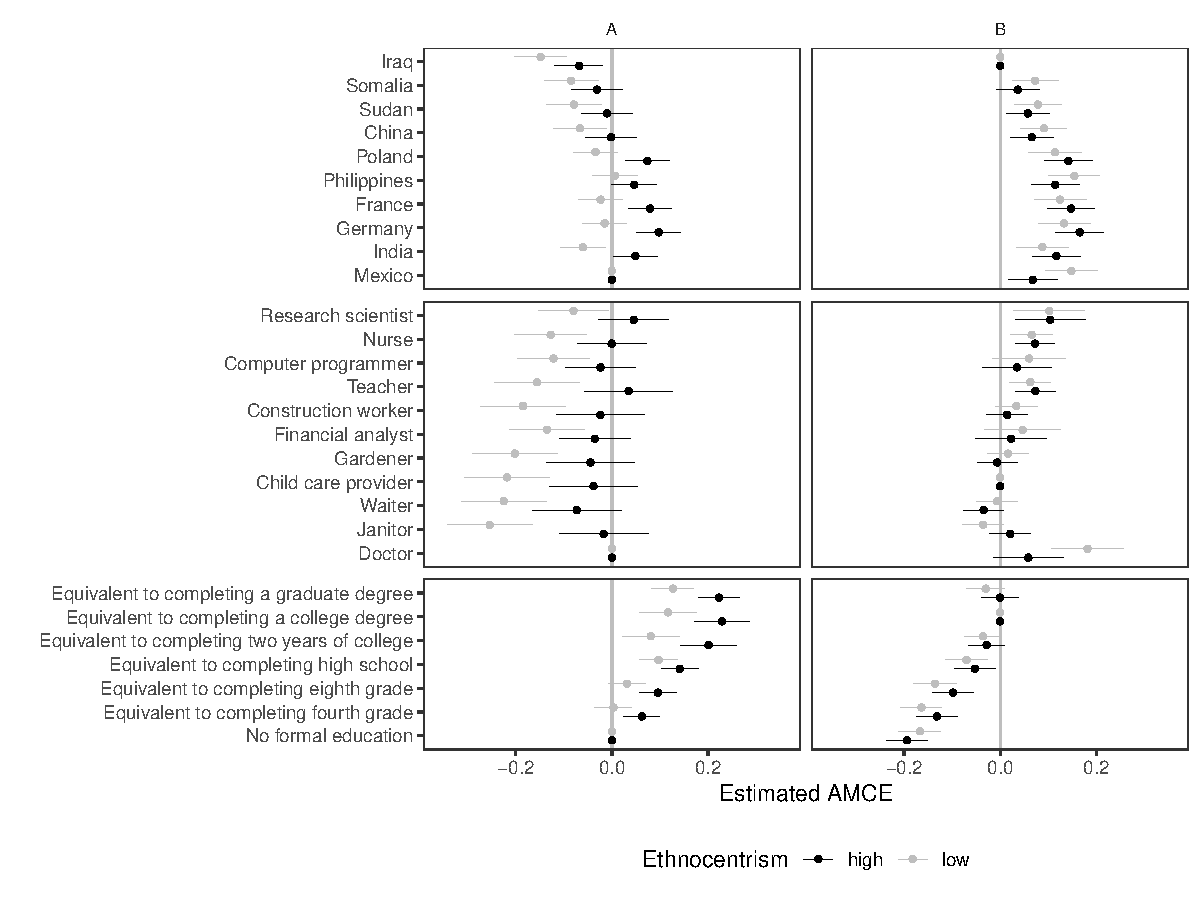
\includegraphics[width=\maxwidth]{figure/hainmueller_subgroup_example_plot-1} 

\end{knitrout}

In our view, the panel B is the more truthful visualization \citep{Cairo2016}. The differences between subgroup AMCEs more accurately convey differences in underlying preferences. Panel A, by contrast, leads the reader to suspect sometimes sizable difference in views along the dimensions of language skills, country of origin, job, and education, among others. 


% higher order margins


\section{Conclusion}\label{sec:conclusion}

This paper has several identified challenges related to the analysis and reporting of conjoint experimental designs, particularly analyses of subgroup differences. It suggests that authors should report not only average marginal component effects (AMCEs) but also descriptive quantities that better convey subgroup differences.

% Present marginal means overall and for specific subgroups of interest
As should be clear from the above discussions, we have relatively straightforward and hopefully uncontroversial advice for how analysts of conjoint experiments should proceed:

\begin{enumerate}
\item Always report unadjusted marginal means when attempting to provide a \textit{descriptive} summary of respondent preferences in addition to or instead of AMCEs. Yet remain cautious about characterizing middling values as ambivalence as opposed to an unobserved pattern of heterogeneity.

\item When choosing reference categories for profile features, do so systematically based upon how the resulting AMCEs will be interpreted. Sensible choices are setting each feature's reference category to the marginal least (marginally most) preferred level, such that all AMCEs for all features are either all positive (negative).

\item Exercise extreme caution when explicitly or implicitly interpreting differences in AMCEs across subgroups given that this quantity is almost always a biased estimate (of unknown sign) of the difference in preferences. If differences in AMCEs are reported, the choice of reference categories should be discussed explicitly and diagnostics should be provided.
\end{enumerate}

% some big conclusion

\singlespacing
\bibliographystyle{apsa-leeper}
\bibliography{references}
\clearpage

\appendix

\section{Additional Results}

The below figure shows full marginal means for high and low ethnocentrism respondents for all feature levels.

\begin{knitrout}
\definecolor{shadecolor}{rgb}{0.969, 0.969, 0.969}\color{fgcolor}
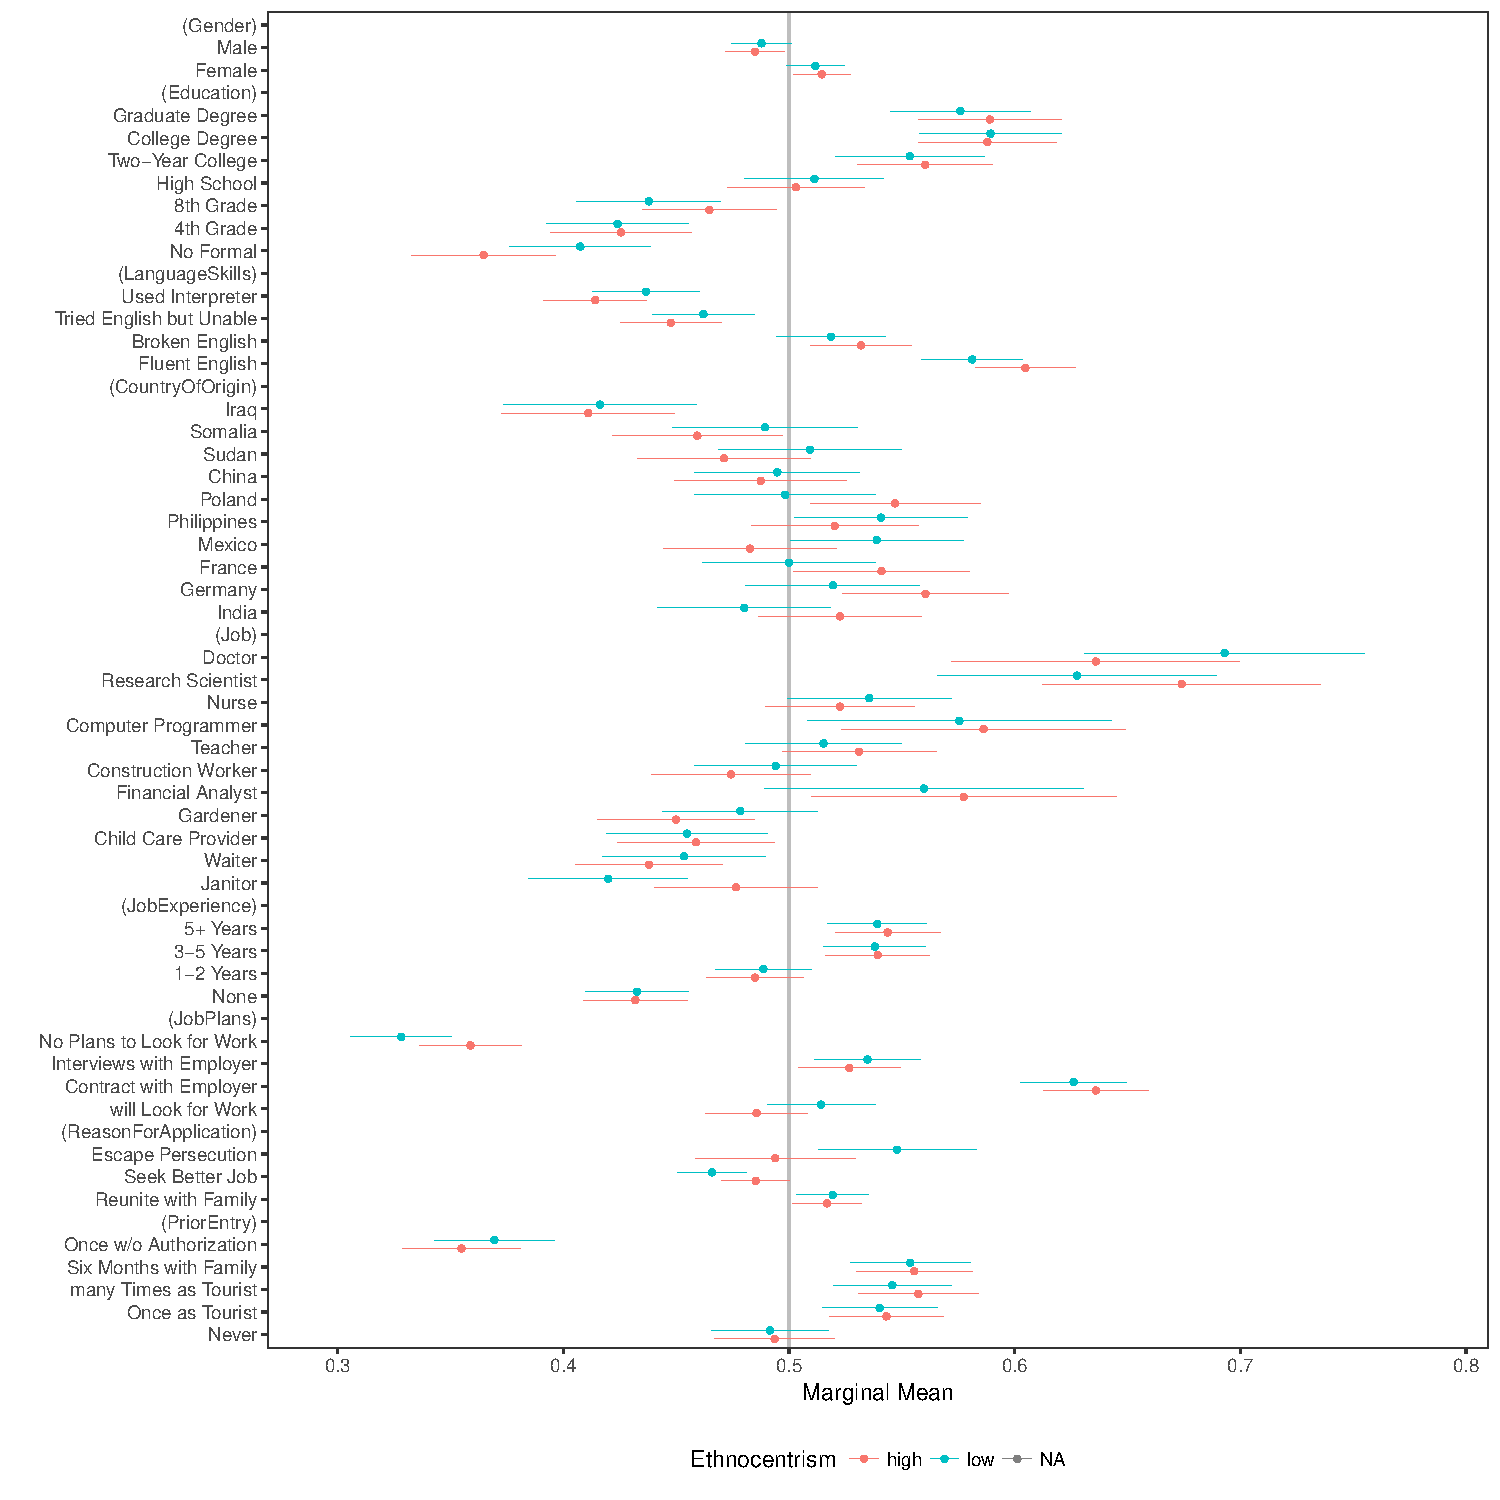
\includegraphics[width=\maxwidth]{figure/hainmueller_mm_by_ethnocentrism-1} 

\end{knitrout}

\end{document}
